\chapter{ALU and ALU Control}

\section{ALU}

First we will build the ALU itself.  The ALU has three inputs (two data inputs to act on, and a control input to determine the action perfomed) and two outputs (one data, and a logical flag). In Figure~\ref{fig:alubits}
\begin{figure}
\caption{ALU control bit meaning.}\label{fig:alubits}
\begin{center}
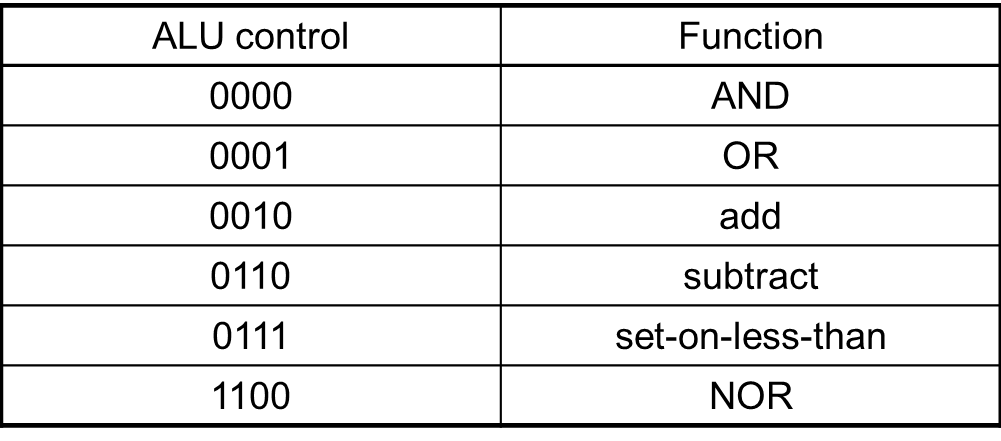
\includegraphics[width=0.6\textwidth]{../images/alubits.png}
\end{center}
\end{figure}
you can see the meaning of the control bits used to determine what the ALU will calculate.  One way to build the ALU is to have it calculate each function and select the one you want.  This is fast and simple but wasteful, thus you would need to determine if speed is a good enough reason to do this.  In our case it is the approach we will take due to the simplicity.  Generating all and selecting indicates a mux, and since there are many options it is a large mux, so a case statement is called for.  The ALU control bits have been given names in the definitions.vh file, so be sure to use them as the individual cases.  Also don't forget to make a default case, which is needed to actually wire this up.  Pick something fast for the default, thus usually a logic statement.

One last thing to note is the generation of the zero flag.  There are several ways to handle this, here are two (you can pick).  
\begin{enumerate}
\item In Verilog (like C), the statement $(a==b)$ is an operation with a boolean output.  You can thus say $x=(a==b);$ to assign $x$ to be the boolean value.  The statement $x=(a==b);$ is realizable as a digital comparator with $a$ and $b$ as inputs and $x$ as the single bit output.
\item Verilog gives you reducing logic by putting the gate before an array of bits, indicating all the bits are to be connected by that logic gate to produce a single output.  This is a particularly elegant gate that is useful in many places including here.  Think how you can determine something is zero by reducing with a gate, then possibly negating.
\end{enumerate}

\section{ALU Control}

Now we need to build the controller to use the ALUOp field and the function field to generate the ALU control bits used above.  Consider the table in Figure~\ref{fig:alucontrolbits}.  
\begin{figure}
\caption{ALU control bit generation.}\label{fig:alucontrolbits}
\begin{center}
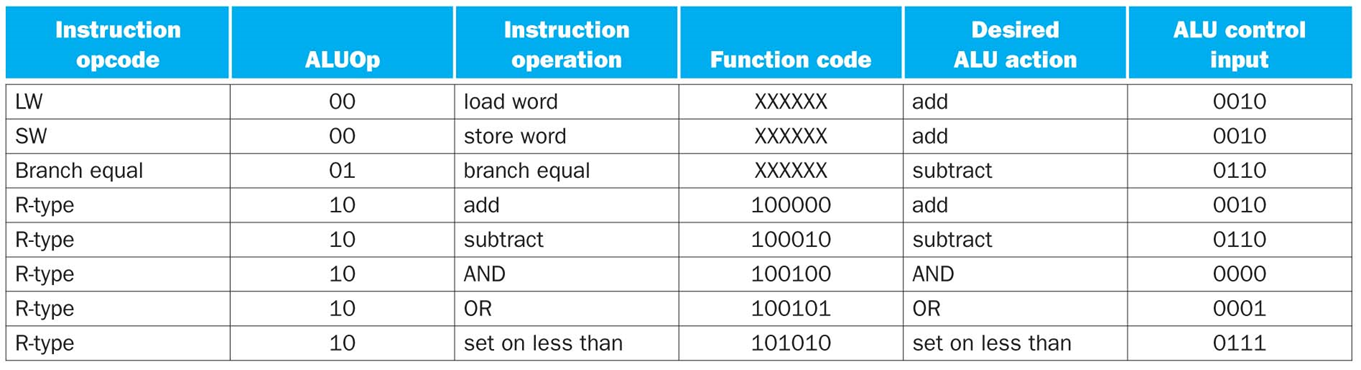
\includegraphics[width=\textwidth]{../images/ALUcontrolbits.png}
\end{center}
\end{figure}
The first two columns are the initial sorting on ALUOp.  The second two columns explain the secondary sorting based on the function field used for R-Type commands.  The final two columns explains what the output of the function should be.  Selecting between many connected values indicates a mux and thus a case statement.  A two layered sorting indicates a nested mux/nested case statement is needed.  Be careful when you code as the nesting is only needed for the R-Type commands.  In both the case statements include a default to handle undefined signals (use fast commands for undefined signals).  Use the signal names defined in the definitions.vh file to improve readability - you shouldn't need any numbers.  This should be a simple module with two inputs (ALUOp and function) and one output (control bits).

\section{Your Assignment}

You are to:
\begin{enumerate}
\item Finish the ALU and ALU control modules.
\item Test both modules with a testbench, run a simulation and generate a timing diagram.
\item  Write up a lab report in \LaTeX\ following the lab format in \verb1LabN.tex1 and generate a pdf file.
\item Upload the pdf and all the Verilog files to the course LMS.
\end{enumerate} 